В рамках диссертационного исследования разработанная нечеткая модель
РС была применена практически при разработке программного
обеспечения, описанию которого посвящен данный раздел.
Как было показано в предыдущей главе, разработанная модель не зависит от
исходных данных, что позволяет создавать на ее основе программное
обеспечение, не привязанное к конкретным исходным данным и
более общего применения, нежели, например, веб-сервис одного конкретного
интернет-магазина. Разработанная модель легла в основу
ядра рекомендательной системы, названного <<Контентный
рекомендательный сервис>>.

Так как модель не зависит от исходных данных, то и разработанное ядро,
основанное на модели, не зависит от того, с каким множеством данных ему приходится работать.
Единственное требование, которые накладывается на исходные данные ---
это требование, накладываемое на структуру базы данных, которая
будет описана ниже. Функция разработанного ядра веб-сервиса заключается
в следующем --- по заданным пользователем характеристикам множества $X$
выполнять поиск интересующих его объектов. То есть функцией ядра является
решение задачи $\top$ при использовании правил вывода нечеткой
контентной модели (\ref{content-solve-tech}).

Так как ядро может работать с любыми исходными данными, то оно может
применяться для любой прикладной области. В рамках диссертационного
исследования было построено программное обеспечение демонстрационных
веб-приложений при применении ядра, множеством объектов
одного из которых является множество музыкальных исполнителей,
другого --- множество фильмов.

Разработанное ядро может быть внедрено в любой веб-сервис, который располагает
базой данных определенной далее структуры.

Ядро системы может дополняться различными модулями, которые расширяют
функциональность системы, что будет продемонстрировано при описании конкретных
двух реализаций.

\section{Структура базы данных}
Требуемая структура показана на рисунке <<Необходимая структура базы данных для
использования ядра>> (\ref{pic:bd-struct}).
\begin{figure}
\caption{Необходимая структура базы данных для использования ядра}
\label{pic:bd-struct}
	\begin{center}[H]
  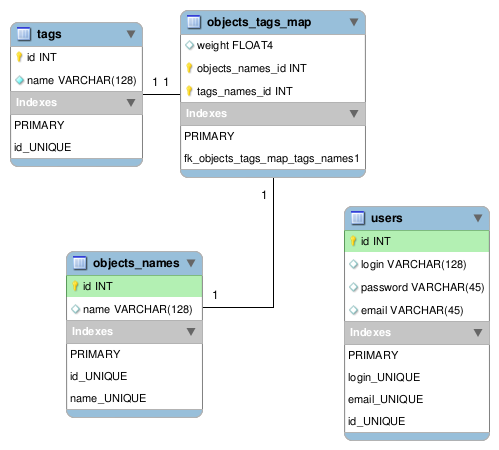
\includegraphics[width=7in,height=8in]{pics/db-scheme-core.png}
\end{center}
\end{figure}

Для работы ядра необходимы следующие таблицы в базе данных:
\begin{itemize}
\item $users$ --- таблица, в которой хранится информация о пользователях. Имеет
	следующую структуру:
  \begin{itemize}
    \item $id$ --- первичный ключ таблицы, целое число;
    \item $login$ --- строка, в которой хранится login пользователя;
    \item $password$ --- строка, в которой хранится пароль пользователя;
    \item $email$ --- строка, в которой хранится email пользователя;
  \end{itemize}
\item $obects\_names$ --- таблица, в которой хранится информация об объектах (objects) предметной области. Имеет следующую структуру:
  \begin{itemize}
    \item $id$ --- первичный ключ таблицы, целое число;
    \item $name$ --- строка, в которой хранится наименование объекта;
  \end{itemize}
\item $tags$  --- таблица, в которой хранится информация о тегах
	предметной области. Теги --- популярный термин, который несет семантику характеристики. Имеет следующую структуру:
  \begin{itemize}
    \item $id$ - первичный ключ таблицы, целое число;
    \item $name$ --- строка, в которой хранится наименование объекта;
  \end{itemize}
\item $objects\_tags\_map$ --- таблица, в которой хранится информация о характеристиках объектов. Имеет следующую структуру:
  \begin{itemize}
    \item $oid$ --- внешний ключ таблицы, связанный с $id$ таблицы $obects\_names$;
    \item $tid$ --- внешний ключ таблицы, связанный с $id$ таблицы $tags$;
    \item $(oid, tid)$ --- пара внешних ключей составляет первичный ключ таблицы;
    \item $weight$ --- вещественное число, являющееся значением характеристики или весом тега;
  \end{itemize}
\end{itemize}

\section{Описание ядра системы}
Ядро системы написано на языке Java с применением технологии Java Servlet-ов,
для использования которых был развернут контейнер сервлетов --- сервер
Apache Tomcat, который позволяет запускать веб-приложения.

Программное обеспечение обладает архитектурой пакетов, изображенной на
UML-диаграммах (\ref{entres-uml1}) и (\ref{entres-uml2}).
\begin{figure}[h]
\caption{UML-диаграмма пакетов ядра}
	\label{entres-uml1}
\begin{center}
  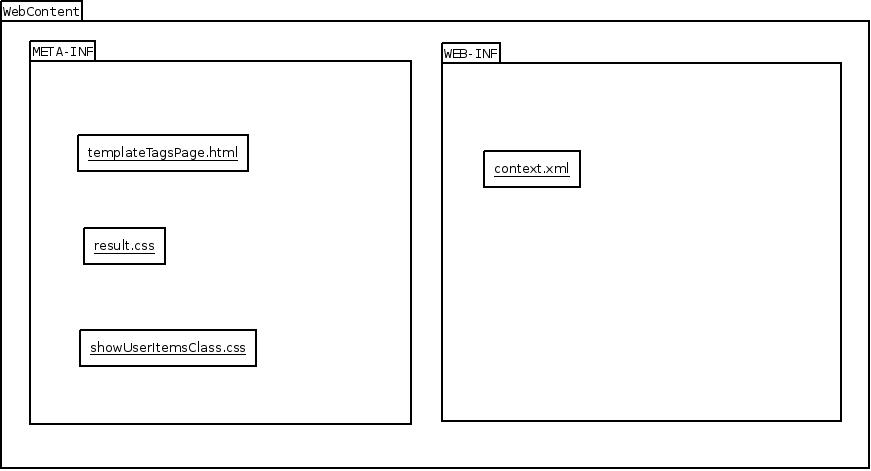
\includegraphics[width=7in,height=7in]{pics/core-web-content.jpeg}
\end{center}
\end{figure}
В Web пакеты ядра входят следующие составляющие:
\begin{enumerate}
\item Пакет <<WEB-INF>>, в котором определены <<.js>> скрипты, стилевые файлы и
	файл-шаблон для предварительных действий, проводимых перед запуском
		системы;
\item Пакет <<META-INF>> содержит файл <<context.xml>>,
	в котором описывается контекст подключения к базе данных.
\end{enumerate}

\begin{figure}
\caption{UML-диаграмма пакетов ядра.}
\label{entres-uml2}
\begin{center}
  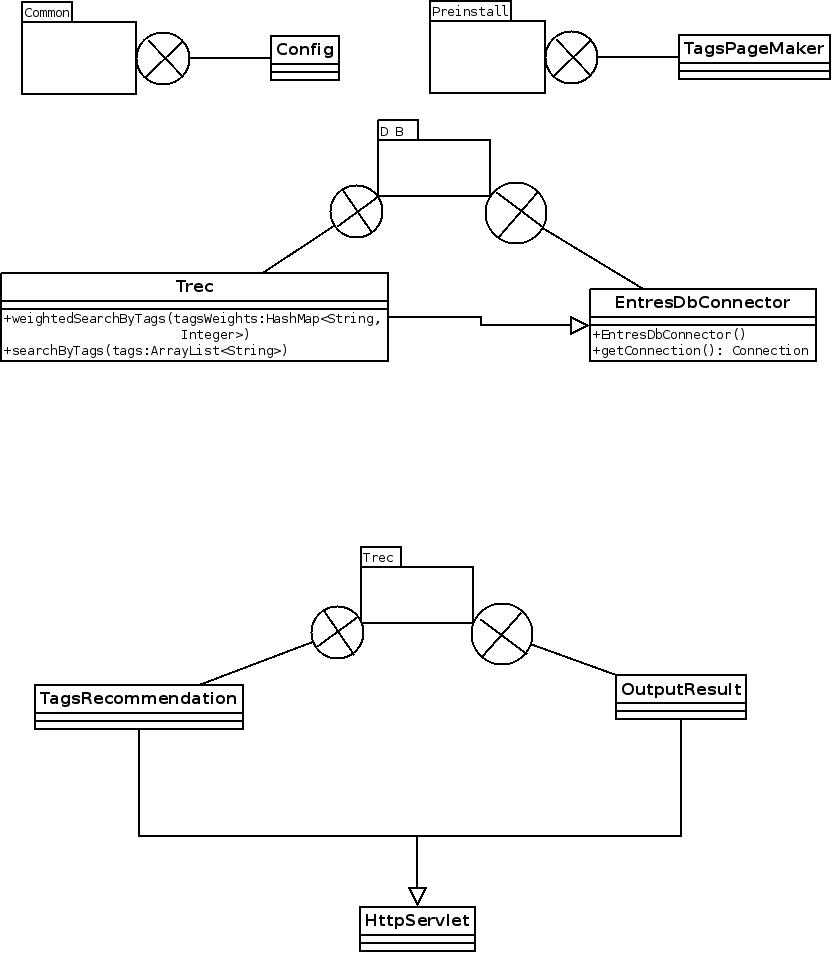
\includegraphics[width=7in,height=10in]{pics/core-packs2.jpeg}
\end{center}
\end{figure}

Ядро системы состоит из следующих пакетов и классов:
\begin{itemize}
	\item Common --- пакет, содержащий общие для всего ядра элементы:
		\begin{itemize}
			\item Класс <<Config>> --- в нем пользователь ядра должен задать
				конфигурационные константы своего приложения, такие, например, как,
				имена таблиц базы данных.
		\end{itemize}
	\item Пакет <<Preinstall>> --- данный пакет содержит классы,
		которые выполняют предварительные действия, необходимые для запуска
		приложения;
	\item <<TagsPageMaker>> --- класс, с помощью которого формируется
		html-страницы веб-сервиса с конcтантным
		  именем <<tagsInputPage.html>>, на которой
		  пользователь может задать теги для поиска интересующих объектов.
		  Страница <<tagsInputPage.html>> формируется по шаблону,
		  входящему в ядро системы --- в пакете WEB-INF,
		  файл <<templateTagsPage.html>>. Это необходимое предварительное
		  действие, необходимое для запуска сервиса, так как ядро не имеет
		  никакой информации о конкретной базе, с которой придется работать.
		  При желании изменения стиля сформированной страницы пользователь ядра
		  может изменить стилевой файл/
	  \item Пакет DB (от Data Base) --- содержит классы, которые осуществляют
		  работу с базой данных. В данном пакете определены следующие классы:
		  \begin{itemize}
			  \item Базовый класс <<EntresDbConnector>>, который описывает
				  подключение к бае данных.
			  \item Класс <<Trec (от Tag Recommendation)>>, наследуемый от
				  класс <<EntresDbConnector>>. В нем определены функции, необходимые ядру
				  для осуществления поиска объектов по заданным тегам. С данным классом осуществляют работу Java-сервлеты после получения данных от пользователя.
				  Класс содержит основные публичные методы:
				  \begin{itemize}
					  \item <<weightedSearchByTags>> --- поиск по тегам,
						  заданных пользователем вместе с указанием их веса;
					  \item <<searchByTags>> --- поиск объектов по списку
						  тегов, заданных пользователем.
				  \end{itemize}
		  \end{itemize}
	  \item <<Trec>> --- данный пакет содержит сервлеты, которые в
		  иерархически
		  находятся между пользователем и базой данных.
		  В пакет входят следующие сервлеты:
		  \begin{itemize}
			  \item <<TagsRecommendation>> --- сервлет, получающий информацию от пользователя и делающий запрос в базу данных
				  на поиск соответствующих объектов через класс Trec пакета DB;
			  \item <<OutputResult>> --- сервлет получающий управление после форвардинга из сервлета <<TagsRecommendation>>. Данный сервлет осуществляет
				  вывод результатов поиска по базе на веб-страницу;
		  \end{itemize}
\end{itemize}

\section{Описание рекомендательного кинематографического веб-сервиса}
На базе ядра было разработано приложение для кинематографиских рекомендаций.
В качестве таблицы $objects\_tags\_map$ использовались данные базы Movie Lens.
В сформированной базе на основе Movie Lens содержится 30 000 фильмов и 200 жанров.
Характеристики объектов могут принимать значения 0 либо 1, в зависимости от того,
принадлежит ли жанр объекту или нет (то есть $w(i, y) \in \{0,1\}$).
В действительности число жанров гораздо больше, но в создаваемом приложении огромное число 
жанров затруднит формирование запроса. Характеристики пользователя совпадают с
характеристиками объекта, то есть $\delta_c(x, y) = 1$.

Помимо основной функциональности была добавлена возможность сохранения пользователем
интересующих его фильмов и просмотр текущего списка. Для этого к базе была
добавлена
дополнительная таблица, что отражено в UML-диаграмме (\ref{pic:db-ml}).

\begin{figure}
\caption{Структура базы данных кинематографического сервиса}
\label{pic:db-ml}
\begin{center}
  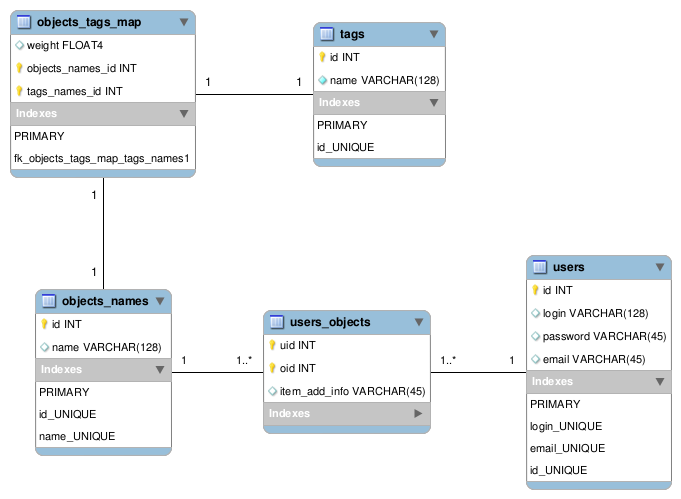
\includegraphics[width=7in,height=6in]{pics/db-scheme-ml.png}
\end{center}
\end{figure}

База содержит дополнительную таблицу $users\_objects$ со следующей структурой:
\begin{itemize}
\item $uid$ --- внешний ключ таблицы, связанный с $id$ таблицы $users$;
\item $oid$ --- внешний ключ таблицы, связанный с $id$ таблицы $obects\_names$;
\item $(uid, oid)$ --- пара внешних ключей составляет первичный ключ таблицы;
\item $item\_add\_info$ --- дополнительная информация, известная о фильме, хранимая в виде строки;
\end{itemize}

Для отображения пользовательской информации был добавлен класс <<ShowUserInfo
>> в пакет Trec, что изображено на следующей UML-диаграмме.
\begin{figure}
\caption{UML-диаграмма пакетов ядра.}
\begin{center}
  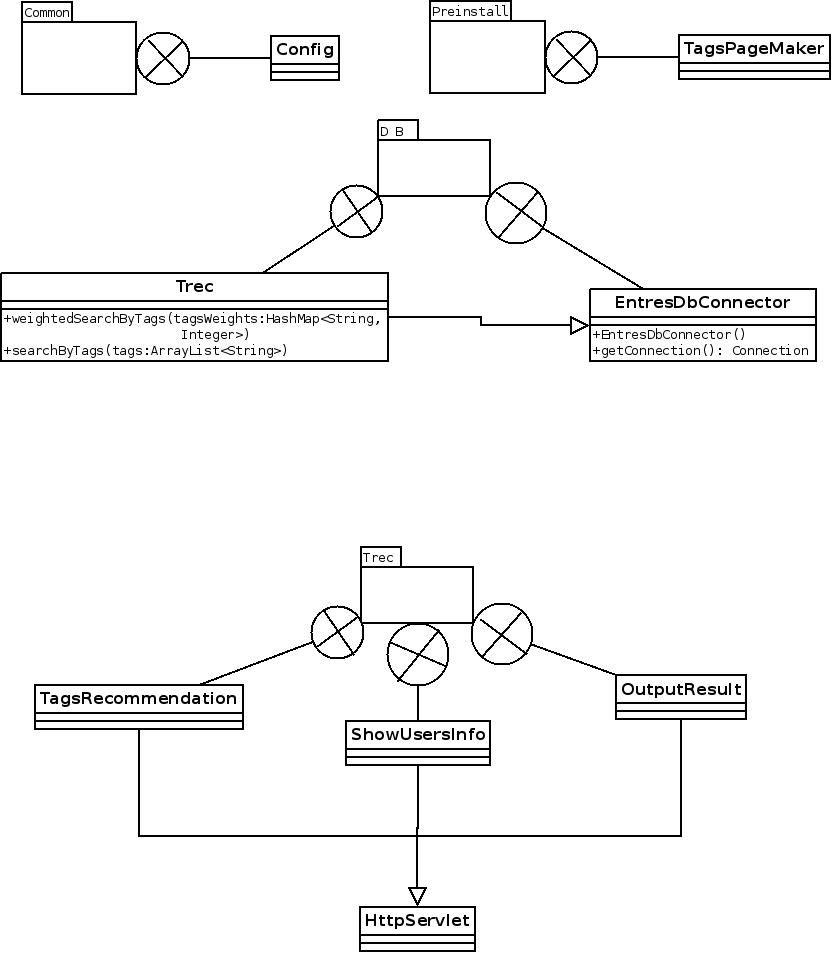
\includegraphics[width=7in,height=7in]{pics/core-packs-ml.jpeg}
\end{center}
\end{figure}

Приведем пример работы с веб-приложением с помощью нескольких скриншотов системы.
На первом скриншоте (\ref{pic:ml-screen1}) виден основной интерфейс пользователя, с помощью которого
он может выбрать интересующие его кинематографические жанры.
\begin{figure}
\caption{Пример выбора пользователем кинематографических жанров для поиска соответствующих им фильмов.}
\label{pic:ml-screen1}
\begin{center}
  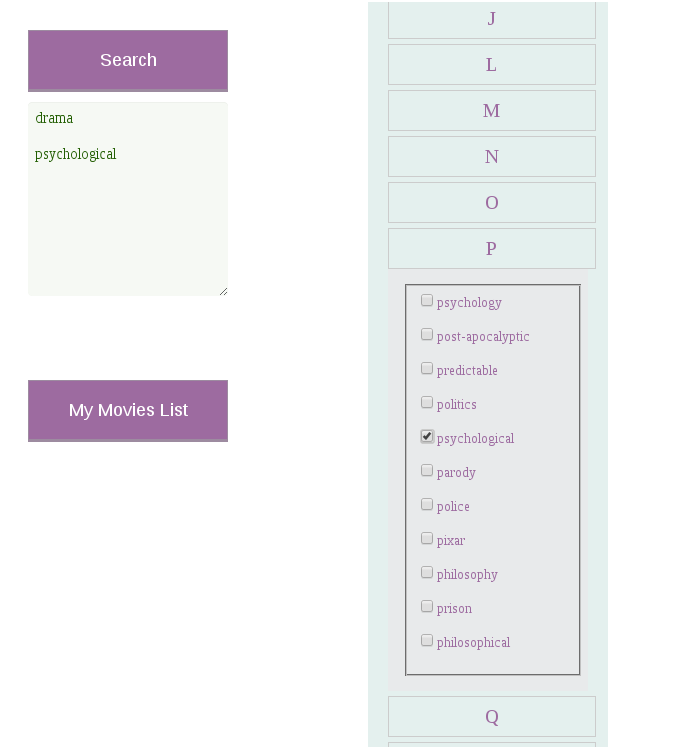
\includegraphics[width=8in,height=9in]{pics/ml-interface.png}
\end{center}
\end{figure}

При задании жанров пользователь формирует собственный контент, значения характеристик принадлежат шкале $\{0,1\}$.
0 --- если пользователь не выбрал жанр, 1 --- иначе. Задача заключается в поиске топовых объектов, поэтому
из базы данных выбираются те объекты, которым принадлежат все выбранные
пользователем характеристик. Результатом
такой выборки являются такие объекты, что $\rho(u_a, i) = 0$.

На скриншоте виден выбор пользователя: его интересуют фильмы, которые обладают
жанрами
<<драма>> и <<психологический>>. На этом же изображении
видна кнопка <<My movies list>>, по нажатию которой пользователь
сможет просмотреть информацию о фильмах, ранее им сохраненных
(см. Рисунок <<Пример списка сохраненных ранее пользователем фильмов>> \ref{pics:save}).
%==========================>
\begin{figure}
\caption{Пример списка сохраненных ранее пользователем фильмов}
	\label{pics:save}
\begin{center}
  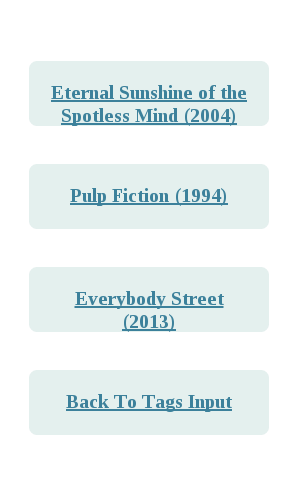
\includegraphics[width=5in,height=5in]{pics/ml-mylist.png}
\end{center}
\end{figure}

На следующем скриншоте (\ref{pic:ml-screen2}) показаны результаты поиска фильмов по запросу пользователя. Если запрос пользователя не устраивает, то
можно сделать повторный и получить другие результаты, нажав кнопку <<Reload>>. Под каждым названием пользователь может
установить галочку и нажать кнопку <<Save Result>>, чтобы занести интересующий его фильм в собственный список.
Так же выводится дополнительная информация о фильме --- IMDB рейтинг. Данная информация сохраняется в колонку  $item\_add\_info$
таблицы $users\_objects$.
\begin{figure}
\caption{Пример результата поиска фильмов}
\label{pic:ml-screen2}
\begin{center}
  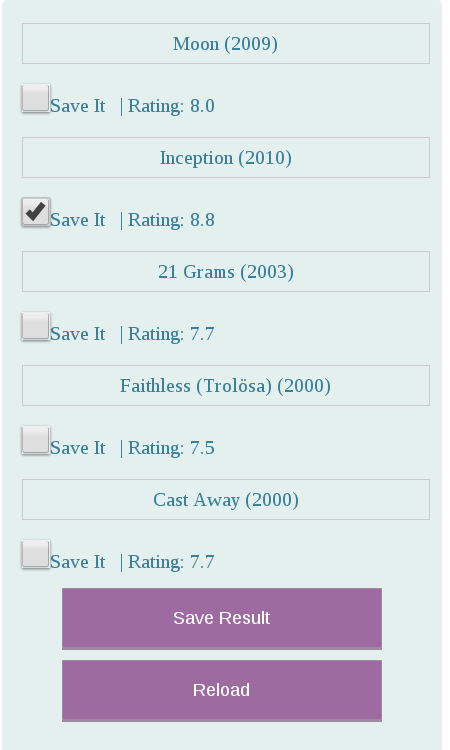
\includegraphics[width=5in,height=5in]{pics/ml-rslt.png}
\end{center}
\end{figure}

\section{Описание рекомендательного музыкального веб-сервиса}
На базе ядра был разработан веб-сервис для поиска музыкальных исполнителей
по заданным пользователям музыкальным жанрам. Музыкальные жанры были
взяты с помощью Last Fm API и среди всего их большого множества оставлены
наиболее
популярные. Всего в базе хранится больше полумиллиона объектов и около 200
самых
распространенных музыкальных жанров. Характеристики пользователя совпадают с
характеристикми объекта.

Созданный веб-сервис имеет дополнительную функциональность, добавленную к ядру:
\begin{itemize}
\item Ведется история выборов пользователей: для этого добавлена таблица $users\_tags$;
\item Существует возможность прослушать понравившееся произведения, отмеченные
	таковыми пользователем ранее. Для этого
добавлена таблица $users\_objects$ и реализован класс <<ShowUserInfo>> в пакете
		<<Trec>>;
\item Вывод результатов сформирован так, что пользователь тут же может
	прослушать найденных исполнителей.
Для этого производится запрос видео на <<Youtube>>, для чего создан класс запроса
		расширенной информации об объекте
<<ExtendedAdditionalQuery>>, входящий в состав пакета <<Trec>>;
\end{itemize}

На следующей UML-диаграмме (\ref{pic:db-lf}) отображена структура базы сервиса.

\begin{figure}
\caption{Структура базы данных рекомендательного музыкального веб-сервиса.}
\label{pic:db-lf}
\begin{center}
  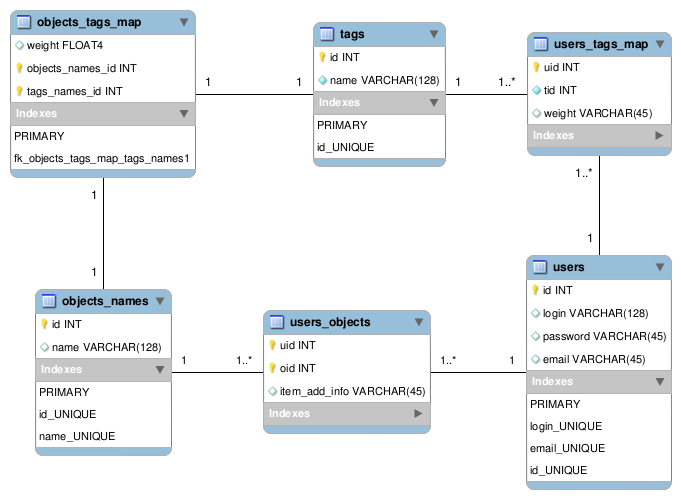
\includegraphics[width=7in,height=6in]{pics/db-scheme-lastfm.png}
\end{center}
\end{figure}

База содержит дополнительную таблицу $users\_tags$ со следующей структурой:
\begin{itemize}
\item $uid$ --- внешний ключ таблицы, связанный с $id$ таблицы $users$;
\item $tid$ --- внешний ключ таблицы, связанный с $id$ таблицы $tags$;
\item $(uid, tid)$ --- пара внешних ключей составляет первичный ключ таблицы;
\end{itemize}

Структура пакетов отображена на следующей UML-диаграмме (\ref{pic:lf-packs}).
\begin{figure}
\caption{UML-диаграмма пакетов ядра}
\label{pic:lf-packs}
\begin{center}
  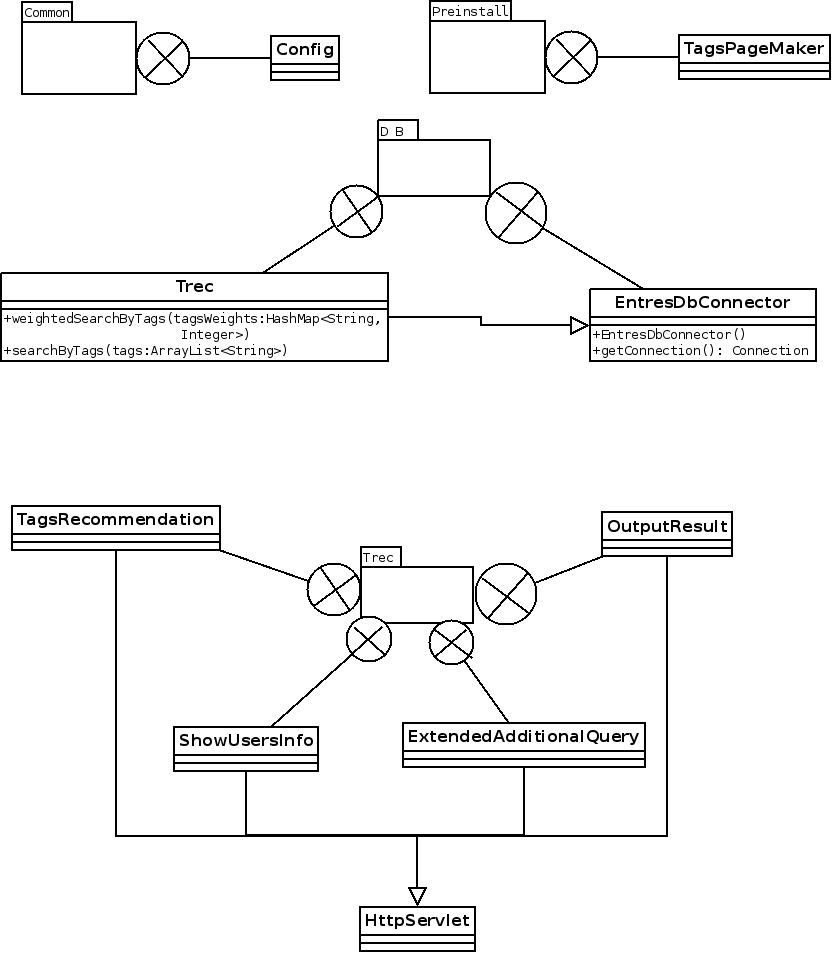
\includegraphics[width=5in,height=5in]{pics/core-packs-lastfm.jpeg}
\end{center}
\end{figure}

Приведем пример работы с веб-приложением с помощью нескольких скриншотов системы.
На первом скриншоте виден основной интерфейс пользователя, с помощью которого
он может выбрать интересующие его кинематографические жанры. Разработанный веб-сервис
имеет более расширенную версию выбора жанров по сравнению с предыдущим сервисом:
пользователь может указать <<вес>> жанра. В терминах нечеткой модели данный вес
отображает степень принадлежности жанра контенту пользователя, который он формирует
при составлении запроса. То есть $w(u,x) \in \{0; 0,3; 0,6; 1\}$. Семантическое соответствие:
\begin{itemize}
\item 0 --- жанр не выбран;
\item 0,3 --- низкая принадлежность;
\item 0,6 --- средняя принадлежность;
\item 1 --- высокая принадлежность.
\end{itemize}
Отображение контета пользователя на множества контентов объектов является тождественным, так как $X = Y$,
но с учетом табицы соответствия значений характеристик пользователя характеристикам объекта $delta_c$:
\begin{table}[h]
\caption{Таблица соответствия характеристик пользователей характеристикам объектов}
\begin{tabular}{|c|c|}
  \hline
  Значение характеристики пользователя & Интервал значений характеристики объекта \\ \hline
  0   & [0; 0,]) \\ \hline
  0,3 &  (0,5; 0,4] \\ \hline
  0,6 & (0,4; 0,7] \\ \hline
  1 & (0,7; 1] \\ \hline
\end{tabular}
\end{table}
К примеру, пользователю с контентом \{(<<Blues>>; 0,8)\} будет
соответствовать объекты, которым принадлежат пары \{(<<blues>>; n)\}, где
$n \in [0,1]$. К примеру, по данному запросу пользователь может получить объект
с именем \{(<<B. B. King>>\}. Таким образом, выбираются объекты,
для которых $\rho(u_a, i) < 0,3$.


На скриншоте (\ref{pic:lf-screen1}) виден выбор пользователя: его интересуют музыкальные исполнители, для которых жанр <<blues>> имеет
высокую принадлежность и жанр <<rock>> --- среднюю.
\begin{figure}[h]
\caption{Пример выбора пользователем музыкальных жанров для поиска соответствующих им исполнителей.}
\label{pic:lf-screen1}
\begin{center}
  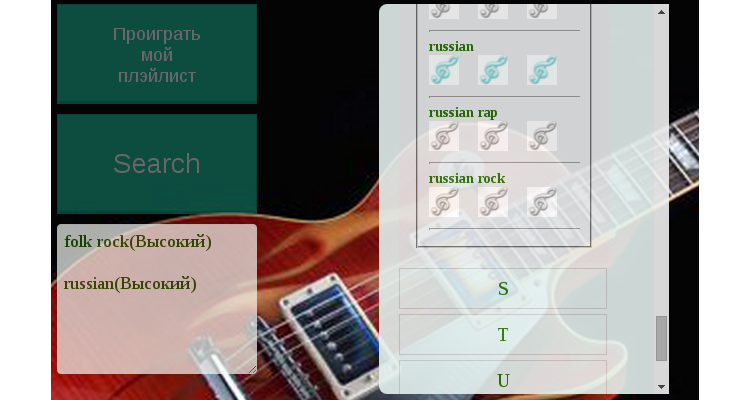
\includegraphics[width=5in,height=3in]{pics/lastfm-interface.png}
\end{center}
\end{figure}

На следующем скриншоте (\ref{pic:lf-screen2}) изображен результат запроса.
\begin{figure}[h]
\caption{Пример результата запроса на поиск музыкальных исполнителей.}
\label{pic:lf-screen2}
\begin{center}
  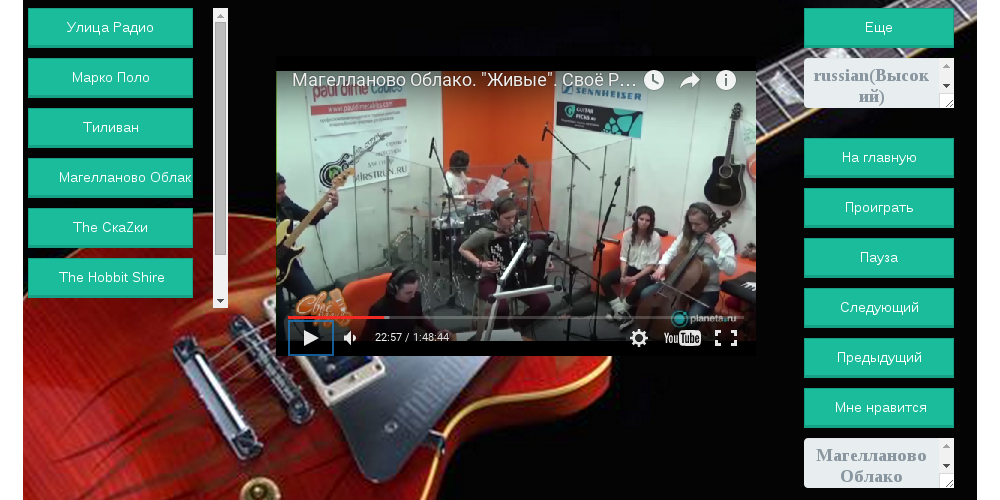
\includegraphics[width=5in,height=3in]{pics/lastfm-rslt.png}
\end{center}
\end{figure}

На скриншоте (\ref{pic:lf-screen2}) видна дополнительная, по сравнению с
предыдущим сервисом, функциональность: можно прослушивать и просматривать
видео исполнителей, выбирая их с помощью навигационных кнопок и сохранять понравившихся в свой плэйлст.

На последнем рисунке <<Пример paylist-a пользователя>> (\ref{pic:lf-screen4}) изображен paylist пользователя. Здесь он может прослушивать понравившиеся и сохраненные ранее им исполнители.
\begin{figure}[h]
\caption{Пример paylist-a пользователя}
\label{pic:lf-screen4}
\begin{center}
  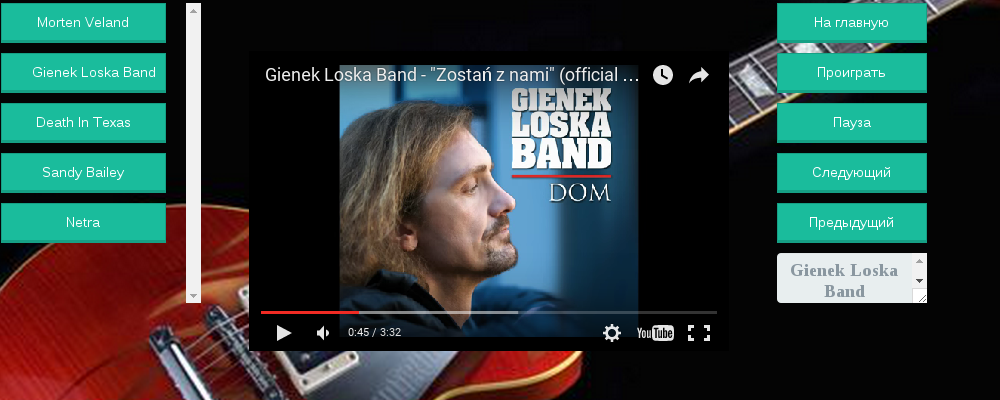
\includegraphics[width=5in,height=3in]{pics/lastfm-mylist.png}
\end{center}
\end{figure}
